\chapter{Introduction}\label{ch:intro}

This thesis presents an approach to the unsupervised learning of morphology (ULM) that 
marries autosegmental theory \citep{mccarthy:1981} and graphical 
computing methods. The novelty of this approach as well
lies in its simplicity and generality. It is equally applicable both to concatenative and 
nonconcatenative morphology, as well as to any language in theory. We will see that
autosegmental theory, once it is distilled down to its essential properties, 
connects quite naturally to graph theory, and hence to graphical approaches 
to machine learning. I will show that a bipartite graphical model in particular, 
because of its a layer of hidden nodes, exhibits the same multilinear properties 
that are behind the effectiveness of autosegmental morphology. 
%Some of this thesis's core ideas were initially explored in \citet{meyer-and-dickinson:2016}. The present work develops these ideas considerably. 
%It also expands and modifies the earlier research.

The power and versatility of autosegmental morphological theory \citep{mccarthy:1981}
stem from its \emph{multilinear} architecture, i.e., its
use of a \emph{segmental tier} along with many \emph{autosegmental tiers} 
to account for morphological structure. The segmental tier is
a series of placeholders for consonants and vowels, often called the
\emph{CV skeleton}. The other tiers each represent a particular \emph{morph}, i.e., unit of morphological structure.\footnote{Our choice of \emph{morph} over another term, such as \emph{morpheme}, is a deliberate  one. The question of what to call the fundamental units of morphological structure is non-trivial, since it is, practically speaking, tantamount to the question of what these fundamental units \emph{are}, i.e., what their nature is. It is thus also very pertinent to the question of what sorts of units can be induced by ULM systems. We will address these questions (as well as motivate our usage of \emph{morph}) in chapter~\ref{autonomous}.}
 
 Figure~\ref{fig:nonlinear} contrasts an autosegmental (or multilinear) morphological analysis  with a linear one, both with respect to the Hebrew word \textit{magdil} (`to make large, magnify').
%The autosegmental analysis for the Hebrew word \emph{magdil} `to make large, magnify.' 
In the autosegmental analysis (figure~\ref{subfig:nonlinear-1}), the morphological structure of \textit{magdil} is represented by four distinct tiers: One is the CV
skeleton, and the other three, labeled $\mu_1$, $\mu_2$, and $\mu_3$, 
correspond to morphs. Each morph is basically shorthand for a particular 
subsequence of phonemes (or graphemes, etc.). Thus, when a morph connects 
with a particular C (or V) in the segmental tier, the C (or V) inherits the 
identity one of the morph's phonemes. For example,  in 
figure~\ref{subfig:nonlinear-1}, $\mu_2$ claims the third phonological 
segment, and thus the third segment takes on the identity of  $\mu_2$'s first phoneme, 
namely /g/. In effect, it \emph{becomes} /g/. 
The morph $\mu_2$ goes on to claim the fourth and sixth segments for its  
%skips the fifth, and claims
%the sixth for its third and final phoneme, 
/g/ and /l/, respectively. It skips over the fifth segment, as it is a V and thus incompatible with its consonantal phonemes.
%The fourth phonological segment likewise belongs to $\mu_2$, 
%so it manifests as $\mu_2$'s second phoneme, namely /d/. Now, $\mu_2$ 
%\emph{does not} claim the fifth phonological segment, as it happens, and thus skips 
%over it, so to speak. It does claim the sixth, however, 
%and thus the sixth phonological segment becomes, in effect, $\mu_2$'s third phoneme, namely /l/. 

The phonemes of $\mu_2$ are thus mapped to phonological segments in 
order: The /d/ in $\mu_2$ must be assigned to a C that follows the 
C associated with /g/, and so on. 
%Likewise, /d/ must be assigned to a C that precedes the C to which /l/ is assigned.
%C associated with /g/. Likewise, the C associated with  is assigned must precede the C associated with 
%/d/, and so on. 
At the 
same, however, the phonemes of $\mu_2$ do not have to be mapped to contiguous \textit{C}s. In figure~\ref{subfig:nonlinear-1}, there is a V between the \textit{C}s associated with the /d/ and /l/, an entirely licit occurrence in Hebrew and other Semitic languages. 
%do not have to be contiguous for the mapping 
%%\textit{C}s or \textit{V}s, and the mapping 
%to work; they could be separated by intervening phonological segments.
%; that can be separated by intervening phonological segments, as indeed are the \textit{C}s associated
%with $\mu_2$'s /d/ and /l/.
%figure~\ref{subfig:nonlinear-1}.
The ability of autosegmental analysis like the one in figure~\ref{subfig:nonlinear-1} to handle such nonconcatenative phenomena is a consequence of the multilinear 
(or autosegmental) architecture of autosegmental morphology \citep{mccarthy:1981}.
%Each morph is essentially an independent data structure  both the ordering of its phonemes as well as 

%In an autosegmental framework, therefore, morphs do not depend on the particular arrangement of phonemes within the segmental string.  of phonological segments.

%morph, or units of morphological structure.
%\footnote{Even though McCarthy uses the term \emph{morpheme} rather than \emph{morphome}, the same principles apply.}

\begin{figure}[t]
%\begin{figure}{R}{0.50\textwidth}
%\vspace{-20pt}
\begin{mdframed}
\centering
	\subfigure[\fontsize{11pt}{12pt}\selectfont Multi-linear approach\label{subfig:nonlinear-1}]{
	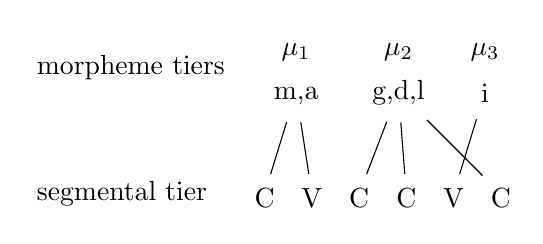
\begin{tikzpicture}[shorten >=2pt,shorten <=3pt, draw=black!100]
	\def \rowthreeht{4.4cm}
	\def \rowtwoht{3.8cm}
	\def \twopointfive{4.1cm}
	%\def \weightstwo{3.75cm}
	\def \rowoneht{2.5cm}
	%\def \weightsone{1.25cm}
	%\def \basement{2cm}
	\tikzstyle{c-node}=[text height=8pt,text centered,inner sep=3pt,minimum size=10pt]
	\tikzstyle{m-node}=[text height=7pt,text centered,inner sep=3pt,minimum size=12pt]
	\tikzstyle{r-node}=[text height=10pt,inner sep=0pt,minimum size=10pt]
	%\tikzstyle{d-node}=[text height=6pt,text centered,inner sep=0pt,minimum size=12pt]
	\tikzstyle{annot}=[text width=25ex,align=left]
	% labels
	\node[annot] (mtierstop) at (0cm,\twopointfive) {morpheme tiers};
	\node[annot] (segtier) at (0cm,\rowoneht) {segmental tier};
	%\node[annot] (mtiersbot) at (0cm,\basement) {};
	
	% surface layer
	\node[r-node] 	(r0)	at (1.0cm,\rowoneht)		{C};
	\node[r-node] 	(r1)	at (1.6cm,\rowoneht)		{V};
	\node[r-node] 	(r2)	at (2.2cm,\rowoneht)		{C};
	\node[r-node] 	(r3)	at (2.8cm,\rowoneht)	 	{C};
	\node[r-node] 	(r4)	at (3.4cm,\rowoneht)	 	{V};
	\node[r-node] 	(r5)	at (4.0cm,\rowoneht)	 	{C};
	
	% hidden-layer elements
	\node[r-node] 	(m0)	at (1.4cm,\rowthreeht)		{$\mu_{1}$};
	\node[r-node] 	(m1)	at (2.7cm,\rowthreeht)		{$\mu_{2}$};
	\node[r-node] 	(m2)	at (3.8cm,\rowthreeht)		{$\mu_{3}$};

	% hidden layer
	\node[c-node] 	(m3)	at (1.4cm,\rowtwoht)		{\/m,a\/};
	\node[c-node] 	(m4)	at (2.7cm,\rowtwoht)		{\/g,d,l\/};
	\node[c-node] 	(m5)	at (3.8cm,\rowtwoht)		{\/i\/};
		
	\path
		(m3)	edge	node	{}	(r0)
		(m3)	edge	node	{}	(r1)
		%
		(m4)	edge	node	{}	(r2)
		(m4)	edge	node	{}	(r3)
		(m4)	edge	node	{}	(r5)
		%
		(m5)	edge	node	{}	(r4);
		
	\end{tikzpicture}
	%\label{subfig:nonlinear}
	}

	\subfigure[\fontsize{11pt}{12pt}\selectfont Linear approach\label{subfig:linear-1}]{
	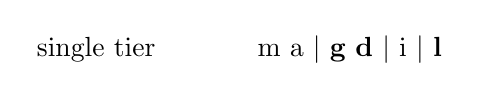
\begin{tikzpicture}[shorten >=1pt,draw=black!100]
	\vspace{50pt}
	\def \floor{0cm}
	\tikzstyle{f-node}=[text centered,inner sep=0pt] %text centered]
	\tikzstyle{annot}=[text width=34ex,align=left]
	% labels
	\node[annot] (floorlabel) at (0cm,\floor) {single tier};
	
	% surface layer
	\node[f-node] 	(f0)	at (1.4cm,\floor)			{m\,\,a\,\,$|$\,\,\textbf{g}\,\,\textbf{d}\,\,$|$\,\,i\,\,$|$\,\,\textbf{l}};
	\end{tikzpicture}
%\label{subfig:linear}
}
\caption{Multiple tiers vs. a single tier for morphological analysis}
\label{fig:nonlinear}
%\vspace{-20pt}
%\vspace{1pt}
\end{mdframed}
\end{figure}

%Notice that $\mu_2$, the consonantal root, is discontinuous; it is
%interrupted by $\mu_3$. 
%This autosegmental account of the 
By contrast, the analysis in figure~\ref{subfig:linear-1} is the \emph{linear} counterpart to the autosegmental  (or multilinear) analysis in figure~\ref{subfig:nonlinear-1}
If a model should have only one tier, as in 
figure~\ref{subfig:linear-1}, there would be no way of representing the
unity of $\mu_2$, i.e., the fact that \textit{g}, \textit{d}, and \textit{l}
all belong to the same morphological unit. Observations such as these motivate this thesis's two principal concepts: \emph{nonlinearity} and \emph{nonsequentiality}. We will define these concepts now and revisit them further in subsequent chapters. 
	\medskip
	\begin{definition}\label{def:nl}{\textbf{Nonlinearity}}: %A model is \emph{nonlinear} 
	A model is \textbf{nonlinear} if each of its morphs occupies a tier that is \emph{not} the phonological tier.
	%Morphs, i.e., units of morphological structure, must be separate from the surface (or phonological) tier. \end{definition} %, i.e., as residing on tiers distinct from the phonological tier. %eparately for m  as being separate from (or outside of) the the phonological (or segmental) tier.  % is a property wherein morphs are represented as being separate from the segmental tier.
	\end{definition}
	\begin{definition}\label{def:ns}{\textbf{Nonsequentiality}}: %is a property such that each morph tier (or node) is orthogonal to all other morph tiers.
	%---i.e., independent of---all other morph tiers. 
	A model is \textbf{nonsequential} if \textbf{no two morphs} occupy the \emph{same} tier. This is to say that all morphs are independent, i.e., that there are no morph-to-morph connections.
	\end{definition}
	\medskip
I propose that these two properties are the essential properties that enable autosegmental morphology to handle nonconcatenative morphology. The main idea of this thesis is that these two properties must be present in any model in order for it to be capable of handling (or learning) nonconcatenative morphology.  We will later revisit the idea stated here as proposition~\ref{prop:nlns} (see in particular section~\ref{sec:framework-intro}).
\begin{proposition}\label{prop:nlns}
%A model of morphology can handle nonconcatenative morphology if and only if it satisfies both \textbf{nonlinearity} and \textbf{nonsequentiality}.
A model of morphology can handle nonconcatenative morphology if it satisfies both \textbf{nonlinearity} and \textbf{nonsequentiality}.
\end{proposition}
%\pex~ Two essential properties  %\ex \label{ex:properties}\begin{xlist}
%	\a {\textsc{Nonlinearity}}: Morphemes are represented as being separate from the segmental tier.
%	\a {\textsc{Nonsequentiality}}: Each morpheme tier (or node) is orthogonal to---i.e., independent of---all other morpheme tiers.
%\xe
% \ex this is one 
%\marginpar{or multilinear}
%These criteria, or essential properties,
%%\textsc{nonlinear} and \textsc{nonsequential} 
%are basically binary variables; each \emph{must} be either True or False, and each can \emph{only} be True or False.  Each variable thus has two possible values,
%giving us four possible combinations of (non)linearity and (non)sequentiality: 
%\textbf{nonlinear nonsequential} (NLNS), \textbf{linear nonsequential} (LNS), 
%\textbf{nonlinear sequential} (NLS), and \textbf{linear sequential} (LS).

%[We should note that autosegmental morphology has other properties to
%constrain morphological structure, e.g., the well-formedness
%principle; at present, we are not concerned with capturing all aspects
%of autosegmental morphology, but instead in building a generic system
%to which one can later add linguistically motivated constraints.]

\section{Research Questions and Objectives}
%State primary research objective: 
%\subsection{Primary research objective}
The primary objective of this thesis is to demonstrate the idea expressed above as proposition \ref{prop:nlns} through a combination of rational argument and experimentation.
%that the crucial components of autosegmental theory, i.e., 
%those components that allow it to handle non-concatenative morphology, 
%This will be accomplished both through rational argument and experimentation.
The rational argument will consist in three main points.
First, the properties of nonlinearity and nonsequentiality are absolutely essential for dealing with nonconcatenative morphology.
Second, these properties are equivalent to the formal mathematical properties that define bipartite graphs. And third, this equivalence provides a foundation for the use of graphical learning models for the purpose of morphological learning. 
%The present study uses a graphical learning framework known as the multiple cause mixture model (MCMM) \citep{saund:94}. 
These points will be further fleshed out in chapters \ref{ch:lit-review}, \ref{ch:graph}, and \ref{ch:MCMM}. These chapters will expand and elucidate concepts originally presented in \citet{meyer-and-dickinson:2016}, an earlier version of the present work.
The experimental component of the dissertation consisted of the development and evaluation of
 \textbf{Multimorph}, a novel unsupervised morphology-learning system that is driven by a Multiple Cause Mixture Model (MCMM) \citep{saund:94} and embodies the three points stated above. 
	
	 \subsection{The Question of Features} There is a great deal of information tacitly present in a string of alphabetic symbols.
	 This is true regardless of whether the string is written, in which case the symbols are graphemes, or spoken,
	 in which case they are phonemes. In either case, the symbols are each drawn from an alphabet of size $N$ and arranged along a single axis.
By way of illustration, consider again the Hebrew word \textit{magdil}, but now specifically as a \emph{string of graphemes}: 
\begin{center}
%\textsf{m\,a\,g\,d\,i\,l}
%\textsf{magdil}
%\texttt{magdil}
%\textipa{magdil}
{\fontsize{12pt}{14pt}\selectfont magdil}
\end{center}
%from figure~\ref{fig:nonlinear}, but now we think of it specifically as the \emph{string of graphemes}.
%\begin{figure}[h]
%\vspace{12pt}
%	\centering
%	\begin{tikzpicture}[shorten >=2pt,shorten <=3pt, draw=black!100]
%	\Large
%	\def \rowoneht{0cm}
%	\def \rowtwoht{-0.8cm}
%	\tikzstyle{r-node}=[text height=10pt,inner sep=0pt,minimum size=10pt]
%	%\node[r-node] 	(r0)	at (0cm,\rowoneht)		{\textipa{magdil}};
%	\node[r-node] 	(r0)	at (0cm,\rowoneht)		{magdil};
%	%\node[r-node] 	(r0)	at (0cm,\rowoneht)		{s t o p};
%	%\node[r-node] 	(r0)	at (0cm,\rowtwoht)		{p o t s};
%	\end{tikzpicture}
%\end{figure} \\
%This row of six graphemes contains a vast amount of tacit information. For instance, suppose we had to represent the string \textit{magdil} not as sequence of alphabetic symbols, but as a series of simple declarative statements. We might come up with statements like the following: 
%%These statements might say that a certain character is present in the string, that one character precedes another character, that a particular character occurs at a particular position in the string, and so on, as in the following examples.
%\begin{itemize}
%  \item \textit{a} immediately follows \textit{m}, \textit{g} immediately follows \textit{a}, \textit{d} immediately follows \textit{g}, and so on. 
%  \item \textit{i} immediately precedes \textit{l}, \textit{d} immediately precedes \textit{i}, and so on.
%     \item \textit{g} follows both \textit{m} and \textit{a}, \textit{d} follows \textit{m}, \textit{a}, and 
%   \textit{g}; \textit{d} precedes both \textit{i} and \textit{l}, \textit{g} precedes \textit{d}, \textit{i}, and \textit{l}, and so on.
%   \item \textit{m} is the first character, \textit{a} is the second, \dots \textit{i} is the second-to-last character, and \textit{l} is the last character, and so on.
%   %\item \textit{l} is the sixth character, \textit{i} is the fifth, \textit{d} is the fourth, and so on.
%   \item \textit{m} precedes \textit{a}, \textit{m} precedes \textit{g}, \textit{m} precedes \textit{d}, \dots, \textit{m} precedes \textit{l}; \textit{a} precedes \textit{g}, \dots , \textit{a} precedes \textit{l}; and so on.
%   \item \textit{m} is present, \textit{a} is present, \textit{g} is present, and so on.
%   \item \emph{ad infinitum}
%\end{itemize}
%A string of alphabetic symbols tacitly conveys all of these facts and many more---perhaps infinitely more.
%Statements like these are essentially what we call \emph{features}.
%Each statement can be either true or false, which is to say that each feature is \emph{binary}, drawn from an alphabet of size $N = 2$.  
%Many machine learning models require that each input object or \emph{learning instance} (in our case, each \emph{word}) be represented as a vector of binary features, not alphabetic features. Moreover, all input objects (learning instances) must be described by the same feature set, and all feature vectors must be of the same length.
%One cannot, of course, have an infinite number of features, as feature vectors must be finite in length.
%Now, let $F$ be the infinite set of all possible features. In keeping with the spirit of my primary research objective, we shall assume that there exists at least one $\phi$ such that $\phi \subset F$, $\phi$ is finite, and $\phi$ allows a ULM system to learn a multilinear model of morphology. The objective here is to confirm this assumption, i.e., to find such a subset.
%There is a great deal of information tacitly present in a string of alphabetic symbols.
%This is true regardless of whether the string is written, in which case the symbols 
%are graphemes, or spoken, in which case they are phonemes. In either case, 
%the symbols are each drawn from an alphabet of size $N$ and arranged along 
%a single axis. % (say, the $x$ axis).
%By way of illustration, consider again the Hebrew word \textit{magdil}, but now specifically as a \emph{string of graphemes}.  In  
%from figure~\ref{fig:nonlinear}, but now we think of it specifically as the \emph{string of graphemes} 
%printed at the top of figure~\ref{fig:many-feats}. 
%By way of illustration, consider the string of graphemes
%displayed at the top of figure~\ref{fig:many-feats}.
%\begin{figure}[h]
%	\centering
%	\begin{tikzpicture}[shorten >=2pt,shorten <=3pt, draw=black!100]
%	\Large
%	\def \rowoneht{0cm}
%	\def \rowtwoht{-0.8cm}
%	\tikzstyle{r-node}=[text height=10pt,inner sep=0pt,minimum size=10pt]
%	%\node[r-node] 	(r0)	at (0cm,\rowoneht)		{\textipa{magdil}};
%	\node[r-node] 	(r0)	at (0cm,\rowoneht)		{magdil};
%	%\node[r-node] 	(r0)	at (0cm,\rowoneht)		{s t o p};
%	%\node[r-node] 	(r0)	at (0cm,\rowtwoht)		{p o t s};
%	\end{tikzpicture}
%\end{figure}
This six-grapheme string contains a vast amount of tacit information. For instance, 
suppose we had to represent the string \textit{magdil} not as sequence of alphabetic 
symbols, but as a series of simple declarative statements. We might come up with 
statements like the following: 
%in in figure~\ref{fig:many-feats}
%\begin{figure}[h]
%%line\hline
%%These statements might say that a certain character is present in the string, that one character precedes another character, that a particular character occurs at a particular position in the string, and so on, as in the following examples.
%\begin{center}
%\Large{magdil}
%\end{center}
%%\smallskip
\begin{itemize}
  \item \textit{a} immediately follows \textit{m}, \textit{g} immediately follows \textit{a}, \textit{d} immediately follows \textit{g}, and so on. 
  \item \textit{i} immediately precedes \textit{l}, \textit{d} immediately precedes \textit{i}, and so on. %What's more, we know that
   \item \textit{g} follows both \textit{m} and \textit{a}, \textit{d} follows \textit{m}, \textit{a}, and \textit{g}; \textit{d} precedes both \textit{i} and \textit{l}, \textit{g} precedes \textit{d}, \textit{i}, and \textit{l}, and so on.
   \item \textit{m} is the first character, \textit{a} is the second, \dots \textit{i} is the second-to-last character, and \textit{l} is the last character, and so on.
   %\item \textit{l} is the sixth character, \textit{i} is the fifth, \textit{d} is the fourth, and so on.
   \item \textit{m} precedes \textit{a}, \textit{m} precedes \textit{g}, \textit{m} precedes \textit{d}, \dots, \textit{m} precedes \textit{l}; \textit{a} precedes \textit{g}, \dots , \textit{a} precedes \textit{l}; and so on.
   \item \textit{m} is present, \textit{a} is present, \textit{g} is present, and so on.
   \item \emph{and so on \dots}
\end{itemize}
%\begin{itemize}
%  \item \textit{\textipa{a}} immediately follows \textit{\textipa{m}}, \textit{\textipa{g}} immediately follows \textit{\textipa{a}}, \textit{\textipa{d}} immediately follows \textit{\textipa{g}}, and so on. 
%  \item \textit{\textipa{i}} immediately precedes \textit{\textipa{l}}, \textit{\textipa{d}} immediately precedes \textit{\textipa{i}}, and so on. %What's more, we know that
%   \item \textit{\textipa{g}} follows both \textit{\textipa{m}} and \textit{\textipa{a}}, \textit{\textipa{d}} follows \textit{\textipa{m}}, \textit{\textipa{a}}, and \textit{\textipa{g}}; \textit{\textipa{d}} precedes both \textit{\textipa{i}} and \textit{\textipa{l}}, \textit{\textipa{g}} precedes \textit{\textipa{d}}, \textit{\textipa{i}}, and \textit{\textipa{l}}, and so on.
%   \item \textit{\textipa{m}} is the first character, \textit{\textipa{a}} is the second, \dots \textit{\textipa{i}} is the second-to-last character, and \textit{\textipa{l}} is the last character, and so on.
%   %\item \textit{\textipa{l}} is the sixth character, \textit{\textipa{i}} is the fifth, \textit{\textipa{d}} is the fourth, and so on.
%   \item \textit{\textipa{m}} precedes \textit{\textipa{a}}, \textit{\textipa{m}} precedes \textit{\textipa{g}}, \textit{\textipa{m}} precedes \textit{\textipa{d}}, \dots, \textit{\textipa{m}} precedes \textit{\textipa{l}}; \textit{\textipa{a}} precedes \textit{\textipa{g}}, \dots , \textit{\textipa{a}} precedes \textit{\textipa{l}}; and so on.
%   \item \textit{\textipa{m}} is present, \textit{\textipa{a}} is present, \textit{\textipa{g}} is present, and so on.
%   \item \emph{and so on \dots}
%\end{itemize}
%\hline
%\end{tikzpicture}
%\caption{Innumerable possible features.}
%\begin{tikzpicture}
%\label{fig:many-feats}
%\end{figure}
%A string like \textit{magdil} tacitly conveys all of these facts and many more---perhaps 
%infinitely more. 
All of these statements, as well as many others,
are tacitly expressed in the string \textit{magdil}.

What we call \emph{features} are essentially true-or-false statements like those listed above.
% ones in figure~\ref{fig:many-feats}.
%Each statement can be either true or false, which is to say that each feature is \emph{binary}, 
%drawn from an alphabet of size $N = 2$.  
Many machine learning models require that each input object or \emph{learning instance} 
(in our case, each \emph{word}) be represented as a vector of \emph{binary} features rather than alphabetic 
features. Moreover, all input objects (learning instances) must be described by the same feature 
set, and all feature vectors must be of the same length.
One cannot, of course, have an infinite number of features, since feature vectors must have a definite length.
One must therefore choose a particular subset of all possible features. The problem of choosing a likely subset constitutes one of
this dissertation's main research questions, and we
%In \ref{ch:intro}, we mentioned the problem of choosing one finite subset of features from an infinite number of possible features.
address it further in chapter~\ref{ch:experi}, where we will glean some insight 
by considering feature categories that 
are significant to computer vision, particularly \emph{invariant} and \emph{variant} features. I will argue that the distinction between these two categories is also important to the unsupervised learning of morphology.
% with an eye to better understanding the sort of features that are valuable to the unsupervised learning of morphology. 
%The idea is that 
%the task of clustering objects, i.e., discerning what makes two objects similar and what makes them different,
%and figuring out which objects to group together and which to separate, is a very general problem. And thus the
%same types of features should apply to different types of objects.
%These categories are \textit{variant} features and \textit{invariant} features. 
%>>>
%We will focus in particular on \emph{invariant} and \emph{variant} features. The distinction between these two categories is highly significant in
%computer vision and its various subfields. For the purposes of this dissertation, we hypothesize that this distinction is
%also important to unsupervised morphological learning. 


\subsection{The Question of Data Representation} 
 %emph{representation} of the input data,
In extracting features from the original data (a list of words), one alters the dataset. Different feature categories emphasize different kinds of information. But the raw material for feature extraction is in any case the original word list, and thus the way in which the words represented in the original dataset plays its own role in shaping features. 
By \emph{representation}, we refer mainly to the alphabet---the
particular set of symbols---from which the strings (i.e., words) of the input wordlist 
are composed.  A word is fundamentally something spoken, i.e., a sequence of sounds, and thus in order to write the word down, one must devise a way to represent the spoken phenomenon on paper. Like feature-set design, this is a means of emphasizing some information at the expense of other information. All else being equal---that is, even if the feature categories are the same---different modes of data representation will produce different features.  
In the present work, three manners of data representation were tested, each presenting 
different information. 

The question of how the input data should be represented is an important one in morphological 
learning because there are often 
a variety ways to represent linguistic data in text form. 
For instance, Japanese can be written in written in \textit{kanji} or 
\textit{kana} characters. The former are entirely logographic, as they 
have been borrowed directly from the Chinese \textit{Han} script, 
and as such, they are not connected to speech sounds in any way. The latter, by contrast,
represent syllables of spoken Japanese. That is, each single \textit{kana} 
character represents both a consonant and a vowel.  (Japanese syllables generally consist of a consonant onset and a vowel nucleus.)  Japanese can also be represented via alphabetic systems, which includes several systems of Romanization as well as scientific phonetic transcription systems such as the International Phonetic Alphabet (IPA).  One might reasonably ask how these various ways of representing Japanese as text might influence the unsupervised learning of Japanese morphology.

%There are indefinitely many ways to represent any language. 
%combination of this two. \textit{Kanji} are logographic characters borrowed directly from the Chinese \texit{Han} script, whereas \textit tAs logographic characters, they are not connected to speech sounds. Japananese   characters and ar chaSome modes of representation 
%are more transcriptional, 
%and others lean toward the orthographic. Some might go to great lengths to capture every phonological and morphophonemic alternation, while others might not express 
%any alternations. Still others might express graphemic alterations; for example, 
%some scripts have different shapes for some letters when the occur word-finally. 
%Some scripts might represent some phonological alternations, but not others, 
%perhaps because those alternations are perceived as more salient than others.
Like that of Japanese, the orthography of Hebrew has a long and rich history. Unlike Japanese, however, Hebrew has never been represented in a non-alphabetic script. Indeed, the ancient Hebrew alphabet was essentially the Phoenician alphabet, the world's first alphabetic writing system and the progenitor of all the alphabets that would in emerge in Europe and the Near East. Still, Hebrew orthography is by no means a straightforward matter, as we shall see in chapter~\ref{ch:experi}.
This dissertation tests three different modes of representing Hebrew as text:
\begin{enumerate}[itemsep=0pt]
\item Transcriptions that mark the primary stress in words
\item Transcriptions without stress markings 
\item Standard Hebrew orthography 
\end{enumerate} 
The third category---the standard orthography---is significant because standard Hebrew 
orthography lacks symbols reserved for vowels. Its alphabet consists only of consonants.\footnote{Some 
consonants can be used to represent vowels, namely the Hebrew equivalents of \textit{w} 
(pronounced as [v] in Modern Hebrew), \textit{y}, and \textit{h}. Even so, these symbols 
are still fundamentally consonants. This and other matters of Hebrew orthography 
will be discussed in chapter~\ref{ch:experi}.} An earlier version of the present work, 
\citet{meyer-and-dickinson:2016}, considered only standard Hebrew orthography. 
We therefore depart from this earlier work in a major way in the present study by including the transcriptional data. 

I initially hypothesized that models induced from the orthographic 
data would be the worst-performing ones. My reasoning was that any orthographic system without dedicated vowel symbols would necessarily let at least some morphologically salient information go unexpressed. I reasoned that this should be especially true in the case of Hebrew, as vowels appear to be especially salient to its morphology. %vowels %appear especially true in the case of Hebrew,  and second, vowels must be particularly important to 
%Hebrew because 
The derivational morphology of Hebrew is famously nonconcatenative, consisting in the interleaving of consonantal 
roots and vowel patterns. The experimental results, however, proved to be somewhat surprising, 
as we shall see in chapter~\ref{ch:results}.
% morphology consist missing out on a great deal of valuable information  It seemed that a vowel-less spelling system would since it seems so obvious that by lacking vowels, it is lacking set wi particularly note this study is noteworthy because the Hebrew alphabet has no vowelsinv take on a different shape word-finally. to a great   to a greater e  The question of data representation determines the raw material from which features are constructed, touches on a number concern the role of the input data in morphological learning, the distinction between information quantity and quality in the input data, as well the influence of 

%transcriptional representations. These differed only in that one marked stress and the other did not. (i.e., all vowels of the t (TS and TR, respectively); The third was \emph{orthographic}, comprising 
%the letters of the standard Hebrew alphabet mapped onto ASCII characters.
%%(\textbf{\text{T}^{S}); another transcriptional, but without stress (\textbf{\text{T}^{R}), and the third orthographic (\textbf{O})ransliterated to ASCII characters in the Hebrew Treebank \citep{simaan-et-al:2001}
%TS is the Berman Longitudinal Corpus's transcriptional system, 
%and TS is that same system with the stress markings removed. 
%%Its alphabet is thus BLC's 
%%transcriptional system, which we discussed above in section. % \ref{sec:transcription}.
%The information contained in O is differs both qualitatively and quantitatively from information contained in the T datasets  
%Arguably, T contains more information than O,
%since T represents each of Modern Hebrew's five vowels in such a way that each 
%vowel sound not only has a symbol, but its own
%has its own exclusive symbol 
%exclusive symbol.

%The features are extracted from raw-text data, wherein Hebrew words are represented as strings of alphabetic symbols, and the symbols are drawn from a particular alphabet. Now, it so happens that we have more than one alphabet at our disposal, and thus more than one way to represent the input data. These alphabets are the following:
%	\begin{enumerate}
%		\item \textbf{Modern Hebrew standard orthography}, as transliterated to ASCII characters in the Hebrew Treebank \citep{simaan-et-al:2001}. In the orthography of Modern Hebrew, certain consonants are regularly appropriated to represent vowels. For example, the Hebrew letter
%		\textcjheb{w}, transliterated as \textit{w} in the Hebrew Treebank, is by default the consonant /v/, but it is also used to represent the vowels /o/ and /u/. In most syllables, however, the vowel is not represented at all. 
%		\item \textbf{Phonemic transcriptions}, i.e., phonemically transcribed words. I have extracted two lists of phonemically transcribed words from the Hebrew portion of the CHILDES database \citep{macwhinney:2000a}. 
%		 These lists are the same except that stress is marked in one, but not in the other.
%	\end{enumerate}
%	%The phonemic transcriptions amount to 12,494 words.
%	The question is which mode of representation yields better feature vectors. This is equivalent to asking which mode delivers the largest quantity of useful information and/or the smallest quantity of irrelevant information.
%	\paragraph{Mixing and Objective Functions.} The \textbf{mixing function} 
%is essentially a voting rule \citep{saund:94}. It prescribes the method whereby the 
%``votes'' of  hidden units are combined to turn a particular feature (i.e., surface unit) \textsc{on} or \textsc{off} (see section~\ref{sec:mixing-function}. The \textbf{objective function} measures the discrepancy---or, alternatively, similarity---between the surface units' activities and their target activities. 
%It thus drives the model's learning by way of trial and error. Objective functions can 
%be either positive or negative. Positive objective functions measure similarity and thus 
%need to be maximized. Negative objective functions measure error and thus need to be minimized (see section~\ref{sec:mcmm-learning}).

%I intend to experimented with two radically different mixing functions, 
%viz. one that combines hidden-unit activities linearly and one that combines them nonlinearly.
%%%(see section~\ref{sec:mixing-function}). 
%Similarly, I intend to try out 
%two radically different objective functions, namely 
%both a negative and a positive % one (see section~\ref{sec:mcmm-learning}).
%objective function. %(see section~\ref{sec:mcmm-learning}).
%Why: What does the mixing function do? What would happen if there were no mixing function? The mixing function maps the hidden-unit activities
%What does the objective function do? What would happen if there were no objective function? 
%If there were no objective function, there could be no learning. Learning proceeds by trial and error. 
%The objective function supplies the error.

\subsection{The Question of Evaluation}  One goal of unsupervised learning is to discover previously unknown categories \citep{parsons:2004}. This is especially true where the present study is concerned. Chapter~\ref{autonomous} argues that unsupervised morphological learners by nature learn \emph{autonomous} morphological units, i.e., units that reside in an independent between phonology and syntax. Such units have no meaning in and of themselves, as they exist independently of syntax and semantics. It is difficult to know going into an experiment what these intermediate categories should look like and what would make purported intermediate categories correct or incorrect. 

%going
%The previously unknown categories in this case are going to be morphological units of some kind.
%However, these units will not be conventional morphemes or morphosyntactic categories. 
%
%Instead, MCMM-generated clusters will correspond roughly to Aronoff's 
%\emph{morphomes} \citep{aronoff:1994}, which can be described as \emph{pre-morphosyntactic} units, i.e.,
%units that have been assembled from phonemes, but have not yet been assigned 
%a syntactic or semantic meaning. I shall use the term \emph{morph} instead of 
%\emph{morphome}, however, since MCMM-generated clusters may not correspond 
%precisely to morphomes in every case (see section~\ref{sec:targets}).

Thus, the evaluation itself presents an important research question, namely the 
question of how to evaluate the output of an unsupervised morphological 
clustering algorithm, particularly one that considers only features of \emph{word-internal form}, 
having no access to word-external morphosyntactic features, e.g., the person, number, 
and gender of surrounding words. In this thesis, therefore, I took a multi-faceted 
approach to the evaluation, that is, one composed of three complementary sub-approaches, 
namely a qualitative, an intrinsic, and an extrinsic component. The extrinsic evaluation 
in particular was designed to address the problems inherent in evaluating an unsupervised 
learning system. This consideration of evaluation as a research question in its own right is 
another point of departure from \citet{meyer-and-dickinson:2016}, which had no extrinsic 
evaluation component, but only an intrinsic component and a much smaller qualitative 
component than that of the present study. We will discuss the evaluation in chapter~\ref{ch:eval}.

%Thus, my system will not require morphological building blocks to have particular
%meanings. Instead, it 
%My system will thus look for \emph{pre-morphosyntactic} 
%units, i.e., ones assembled from phonemes, but not yet assigned 
%a syntactic or semantic meaning. In a larger pipeline, such 
%building blocks could serve as an interface between morphosyntax 
%and phonology. For instance, while an MCMM can find Hebrew's default 
%masculine suffix \textit{-im}, it cannot say whether it is
%masculine or feminine in a given word, as this suffix
%also occurs in idiosyncratic feminine plurals. The extrinsic part of the evaluation will examine my system's utility as a component within such a pipeline
%(see section~\ref{sec:paradigms}).
%\emph{morphs}. \marginpar{I have yet to introduce morphs, tho} We do not know 
%beforehand \emph{exactly} what these morphs ought to look like. Since we cannot know 
%the ``right answers'' before the experiments are run, there can be no clear gold 
%standard against which to evaluate the MCMM's output. 
%
%Thus, the evaluation itself presents an important research question, namely the question of how to evaluate the output of an unsupervised morphological clustering algorithm, particularly one that considers only features of \emph{word-internal form}, having no access to word-external morphosyntactic features, e.g., the person, number, and gender of  surrounding words. Such an algorithm will inevitably produce clusters that do not correspond to abstract morphosyntactic categories or conventional morphemes.
%which are fundamentally morphosyntactic in nature even though the correspondence between morphemes and abstract, or ``atomic,'' morphosyntactic categories is not always one-to-one.

\section{Organization}
The remainder of this thesis is organized as follows: In chapter~\ref{ch:lit-review}, 
I present a new framework for thinking about the unsupervised learning of morphology. 
This framework is original to this thesis and stems from the concepts of nonsequentiality 
and nonlinearity, introduced above as the essential prerequisites for modeling 
nonconcatenative morphology. Chapter~\ref{ch:graph} establishes the relationship 
between autosegmental morphology and graph theory, particularly \emph{bipartite} 
graphs. Chapter~\ref{ch:MCMM} then introduces and describes a particular bipartite 
graphical learning model, namely the Multiple Cause Mixture Model (MCMM). 
As mentioned above, this is the learning model I have chosen to drive Multimorph, 
the system developed in this dissertation. The first four chapters thus establish a logical 
chain linking autosegmental morphological theory to a particular unsupervised learning 
model, namely the MCMM, which serves as Multimorph's learning model. 

The remaining five chapters (chapters \ref{autonomous} through \ref{ch:conclusion}) 
are concerned with the evaluation of Multimorph. Chapter~\ref{autonomous} addresses 
the question of the sort of categories that Multimorph and other unsupervised morphological 
should be expected to learn, i.e., the sort of categories that one should look for in evaluating such 
systems. This is part of the question of evaluation introduced above. Chapter~\ref{ch:experi} 
%describes the experimental setup;
describes the choices for Multimorph's features and the preparation of its datasets, thus addressing the questions of features and data representation.
%describes the preparation of Multimorph's input
%that is, it describes the collection and preparation of the datasets 
%and the experimental variables, including the three modes of data representation and the 
%parameters for the feature sets.
 Chapter~\ref{ch:eval} completes this thesis's response to the 
``question of evaluation.'' It describes a dual-paradigm evaluation method consisting of 
both an intrinsic and extrinsic component. The extrinsic component in particular may be 
of interest to other ULM researchers as an alternative to conventional evaluation methods. 
The results are presented and discussed in chapter~\ref{ch:results}, and chapter~\ref{ch:conclusion} 
offers concluding remarks.